%%%%%%%%%%%%%%%%%%%%%%%%%%%%%%%%%%%%%%%%%%%%%%%%%%%%%%%%%%%%%%%%%%%%%%%%%%%%%%%%
\begin{frame}{Supercapacitors}

\begin{columns}
\column{0.6\linewidth}
\includegraphics[width=\linewidth]{rawfigs/supercapacitor/ragone_plot}
\column{0.3\linewidth}
\tiny
\includegraphics[width=\linewidth]{rawfigs/supercapacitor/simplified_ragone_plot}

From [M. Winter and R. Brodd, Chem. Rev., \textbf{104}(10), 4245-4270 (2004)]

\end{columns}
\end{frame}

%%%%%%%%%%%%%%%%%%%%%%%%%%%%%%%%%%%%%%%%%%%%%%%%%%%%%%%%%%%%%%%%%%%%%%%%%%%%%%%%
\begin{frame}{Governing equations in the porous electrode}

\begin{columns}
\column{0.45\linewidth}
\begin{block}{Solid phase $\Omega_1$}
\tiny
\begin{align*}
\nabla \cdot i_1 = 0 \\
i_1 = -\sigma \nabla \Phi_1
\end{align*}
\end{block}

\begin{block}{Liquid phase $\Omega_2$}
\tiny
\begin{align*}
\frac{\partial c_j}{\partial t} = - \nabla \cdot N_j \\
N_j = -D_j \left( \nabla c_j - z_j \frac{F}{RT} c_j \nabla \Phi_2 \right) \\
\nabla \cdot i_2 = 0 \\
i_2 = F \sum_j z_j N_j \\
\sum_j z_j c_j = 0
\end{align*}
\end{block}

\column{0.45\linewidth}
\begin{center}
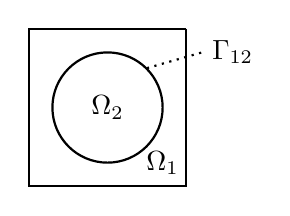
\begin{tikzpicture}
\draw[black,thick] (1,1) -- (1,-1) -- (-1,-1) -- (-1,1) -- (1,1);
\draw[black,thick] (0,0) circle (0.7);
\draw node at (0,0) {$\Omega_2$};
\draw node at (0.7,-0.7) {$\Omega_1$};
\draw[black,thick,dotted] (0.5,0.5) -- (1.2,0.7) node[anchor=west] {$\Gamma_{12}$};
\end{tikzpicture}
\end{center}

\begin{block}{Solid-liquid interface $\Gamma_{12}$}
\tiny
\begin{align*}
i_n = C \frac{\partial \eta}{\partial t} + f(\eta, c_j) \\
f(\eta, c_j) = i_0 \left[ \exp\left( \frac{\alpha_a F}{RT} \eta \right) - \exp\left( -\frac{\alpha_c F}{RT} \eta \right) \right] \\
\eta = \Phi_1 - \Phi_2 \\
i_2 \cdot n = -i_1 \cdot n = i_n \\
z_j F N_j \cdot n = -\frac{d q_j}{d q} i_n
\end{align*}
\end{block}
\end{columns}
\end{frame}

%%%%%%%%%%%%%%%%%%%%%%%%%%%%%%%%%%%%%%%%%%%%%%%%%%%%%%%%%%%%%%%%%%%%%%%%%%%%%%%%
\begin{frame}{Electrochemical impedance spectroscopy}
%\begin{itemize}
%\item A powerfull tool to characterize energy storage devices
%\item Measure the response of the system to AC excitation signals over a broad
%      range of frequencies
%\item Compare against equivalent circuit models
%\end{itemize}
\includegraphics[width=0.6\linewidth]{rawfigs/supercapacitor/comparison_supercapacitor_vs_equivalent_circuit}

\includegraphics[width=0.6\linewidth]{rawfigs/supercapacitor/bode_plot_no_faradaic_processes}
\includegraphics[width=0.35\linewidth]{rawfigs/supercapacitor/nyquist_plot_no_faradaic_processes}
\end{frame}
